\documentclass[10pt,a4paper]{article}
\usepackage[utf8]{inputenc}
\usepackage{amsmath}
\usepackage{amsfonts}
\usepackage{amssymb}
\usepackage{a4wide} %Wider margins
\usepackage[english]{babel} %English dictionary for hyphenation and definitions, e.g. Table vs. Tabel
\usepackage[official]{eurosym} %Support for Euro-sign
\usepackage[utf8]{inputenc} %Support for internationalization, e.g. é vs.\’e
\usepackage{amsmath,amssymb,amsthm} %Support for mathematical formulas and symbols
\usepackage{fancyhdr} %Fancy headers
\usepackage{hyperref} %Creates clickable links
\usepackage{graphicx} %Support for grahpics
\usepackage{nopageno} %Support for removal of pagenumbers
\usepackage{tabularx}
\usepackage{enumitem}
\usepackage{xspace}
\usepackage{algorithm,algpseudocode}
\usepackage{float}
\usepackage{mathtools}
\usepackage[dvipsnames]{xcolor}
\usepackage[titletoc,toc,title]{appendix}
\usepackage{listings}
\usepackage{makecell}
\graphicspath{ {./ThesisFigures/} }

\hypersetup{
    pdftitle={}, %PDF-file will be given a proper title when viewed in a reader
    hidelinks %PDF-file will be given clickable, yet not visible links when viewed in a reader
}
\newcommand{\documenttitle}{TPOT's performance for Biomedical Data}
\newcommand{\documentsubtitle}{A Data Mining Seminar}


\newcommand{\true}{{\sc True}\xspace}
\begin{document}
	
	\begin{titlepage}
		
		\center
		
		\vspace*{3cm}
		
		\textbf{\huge \documenttitle}
		
		\textit{\LARGE \documentsubtitle}
		
		\vspace*{2cm}
		
		\large
		\centering
		T.P.A.~\textsc{Beishuizen}~(0791613)\\
		Biomedical Engineering - Computational Biology\\
		Data Engineering - Information Systems\\
		Eindhoven, University of Technology\\
		Email: \texttt{t.p.a.beishuizen@student.tue.nl}
		
		\vfill
		
		\vspace*{1cm}
		
		\today
		
	\end{titlepage}
	
	\tableofcontents
	
	%\newpage
	
	\pagestyle{fancy}
	%Abbreviations used by fancyhdr:
	%E Even page
	%O Odd page
	%L Left field
	%C Center field
	%R Right field
	%H Header
	%F Footer
	\fancyhead{} % clear all header fields
	\fancyfoot{} % clear all footer fields
	\renewcommand{\headrulewidth}{0.4pt}
	\renewcommand{\footrulewidth}{0.4pt}
	
	\fancyhead[L]{\rightmark}
	\fancyfoot[C]{\thepage}
	\fancyhead[R]{T.P.A. Beishuizen}
	
	
	\clearpage
	
	\section{Introduction}
	\label{sec:Introduction}
	
	% Quick explanation for biomedical data
	At the Computational Biology department (cBio) of Biomedical Engineering (BME), many requests are made to analyse gathered data. This data usually stems from research in hospitals, but can also be from other BME groups and publicly available data. Currently a standard is missing to efficiently analyse those data sets. With the vast number of data sets that are available, such a standard in the form of a framework on data analysis would be valuable. It would speed up projects and give them a higher chance to succeed the goal, due to improved efficiency.
	
	% Explanation skin disease data
	An example of biomedical data sets was based around gene expression of skin diseases. Two skin diseases were tested, psoriasis and atopic dermatitis, the latter one better known as a form of eczema. The expression of a big number of genes was tested for skin disease patients on skin affected by the disease (lesional skin) and skin not affected by the disease (non-lesional skin). At last there were normal patients, that did not suffer from the skin disease. Nine data sets were available for these data set, six for psoriasis and three for atopic dermatitis. The number of tested skin plaques ranged from 28 to 180 whereas the number of tested genes is the same for every set, namely 54675.
	
%	% Quick explanation bariatric data
%	An example of biomedical data sets from cBio stemmed from the Catharina Hospital in Eindhoven. This extensive data set was a combination of two data sets. The first is a data set filled out by a doctor that analysed basic human features as well as the presence of co-morbidities. The second data set consisted of 41 markers measured pre- and post-surgery for 2367 patients that underwent gastric sleeve or gastric bypass surgery, also known as bariatric surgeries. The number of bariatric surgeries is increasing worldwide. Although initially thought otherwise, this type of surgery has added benefits on top of losing weight. Among those benefits the remission of metabolic co-morbidities can be named. Due to binary labelling of those co-morbidities, valuable information is lost. On top of that the labelling is not clearly defined either. To obtain more and better results, this binary labelling could be replaced by a continuous severity score. Ruben Deneer conducted a research on trying to achieve a successful replacement. This data set is a prime example of a data set that is not trivially preprocessed, when looking at multiple data sets, missing values and erroneous data.\cite{Deneer2017Thesis}
	
	% Quick explanation for automated machine learning
	A possible solution for partly providing a framework for cBio can be found in automated machine learning (autoML). This relatively new extension to machine learning tries to automatically search the best combination of preprocessing, feature selection and machine learning algorithms to efficiently describe a data set. CPU or actual time and memory usage are the two main constraints for autoML, due to testing different methods with varying parameters taking up time and space. These autoML algorithms usually are made with the combined algorithm selection and hyperparameter optimization (CASH) challenge in mind.\cite{feurer2015efficient} 
	
	% Introduction of TPOT
	Olson and Moore proposed a tool for autoML, a Tree-based Pipeline Optimization Tool (TPOT).\cite{olson2016tpot} This tool also tries to find the best classifier by creating pipelines for the different algorithms. The pipelines are evaluated and branched or altered according to the evaluation. It makes use of genetic programming, a technique used for evolutionary computations.\cite{banzhaf1998genetic} Evaluation of several TPOT approaches are proven better than doing a basic machine learning analysis and are therefore a promising approach for implementation.\cite{olson2016evaluation} Several projects used layering and meta-learning techniques to tackle the time and space constraints.\cite{Gijsbers2017Thesis}
	
	% TPOT and biomedical data
	To test if TPOT is also suitable for biomedical data, it must be tested by a specific set, such as the bariatric data set. This data consists of several biomedical data challenges only some of which seem solvable by TPOT. A research must be done to find out whether TPOT can manage to retrieve good results from this data set and may benefit of some improvements.
	
	% Layout data seminar
	For the data seminar, first the background will be given. This background will be about the biomedical data sets, the exemplary data set used for the seminar, a topic of automated machine learning and at last a part about TPOT. Secondly the research question is given, together with a hypothesis.
	
	\section{Background}
	\label{sec:Background}
	
	\subsection{Biomedical data}
	
	\label{subsec:BiomedicalData}
	
	% Biomedical engineering description.
	Biomedical engineering can be seen as a specific part of engineering with a wide variety of topics. These topics can be theoretical, non-experimental undertakings, but also state-of-the-art applications. Not only research and development can be used, but also implementation and operation. Combining all of these different parts in one definition is hard.\cite{bronzino2014biomedical} For this project, the focus is mainly on research and development, also known as knowledge discovery.\cite{bramer2007principles} 

	% Biomedical research summary
	When a biomedical engineer starts a project, at the start usually only a data set and the research goal are known. To achieve that certain goal from the data set, four aspects influence the project's course and development. At first obviously the data itself is a big part of such an influencer as the research is restricted to limitations from it. Examples of such restrictions are multidimensionality, set size, data heterogeneity, missing feature values and population handling. The other obvious influencer is the main research goal. Since the biomedical engineer wants to achieve a certain goal, the approach outcome must match that goal for the research to be successful. Most goals are focused around either data mining, extracting relations from available data, or modelling, creating a model within data features. A third influencer is the availability of data analysis tools. The steps to take from data to goal do not only include an approach, but also a tool to execute it. The choice of a certain tool has a big impact on the project, as each one of them has its own advantages and disadvantages. The two most well known tools within BME are MATLAB and Python, however some engineers have used R, Java or C++ and there are still other possibilities. A last big influencer is the biomedical knowledge. What experience the scientist already has with similar projects can greatly influence the choice of approach and framework. Knowledge of the supervisor and publicly known information on the research subject from books and articles also influence the approach, as already known outcomes do not have to be researched again. 
	
	% Process steps for biomedical research
	For data engineers the main focus lies in trying to find patterns in the data. Therefore in this seminar the focus will mainly be on the data driven aspect of a biomedical project. Characteristics of such a data driven approach (as mentioned before) are mainly focused around data volume, dimensionality, complexity, heterogeneity and quality.\cite{chen2006medical, doi:10.1093/bib/bbx044}
	
	% Volume challenge
	Collecting data because it is possible can make data sets bigger than needed. Both in number of instances and features, data sets can be harder to understand or analyse when more is available.\cite{chen2006medical} This volume problem usually is tackled by taking sub-populations of the complete set. These sub-sets can either be focused around a part of the population (gender, age, race) or taken at random to still represent all of it. Due to the efficiency of analysis techniques and the rise in computational speed of servers\cite{blythe2008rise}, volume on its own becomes less of an issue. Volume does however become an issue when combining with heterogeneity and quality.\cite{Turkay2014, Holzinger2014} 
	
	% Dimensionality challenge
	Not all data sets have a high number of instances that cause a big data volume. Sometimes there are relatively few instances, while the number of features is proportionally high.\cite{dubitzky2007fundamentals} Usually many of those features are not relevant enough for the research, however are still used for testing. Trying to remove features that are not important, will greatly help finding relations between the others and create more knowledge about the research topic. Lowering the number of features also makes the data volume go down, so analysis should be easier. Mainly an optimal features set should be selected to obtain the best results.\cite{PENG201015}
	
	% Complexity challenge
	Biomedical data can also be very complex. Useful results may be present, however it can be very hard to obtain it. Examples of complex data are images, several biomedical signals and temporal data. Details of the useful results that are present in images can for example be very hard to detect, the temporal data can vary quite much over time and the biomedical signals can be hard to combine with static biomarkers.\cite{Yoo2012} This aspect can benefit from exchanging knowledge with other research areas that specialize in mining of those complex data sets.\cite{Turkay2014, bellazzi2011data}
	
	% Heterogeneity challenge
	The biggest challenge encompasses aligning different data sets. No standard for data sets is available and therefore data sets differ greatly from each other. Data is weakly structured or even unstructured\cite{Holzinger2014} and variables are processed differently due to other protocols or the collectors' preference of representation.\cite{Otasek2014} Also the variety of data is hard to combine when sources are fundamentally different. When parts of the data are images, another part is a table from the laboratory and a third part is textual remarks of the doctor, standardizing merging those three is much harder than merging three lab sets. Those merges are also very prone to errors, as imprecisions can be vastly different between those data sets. No tool can work directly with these raw data sets and preprocessing must almost definitely occur beforehand.\cite{Turkay2014, CIOS20021}
	
	% Quality challenge
	A last challenge is about data quality. The data is usually gathered by doctors and laboratory workers. Since the data is manually gathered by humans, the data have a relatively high error rate. Therefore the data can be quite noisy, values can be inconsistent, wrongly entered or even missing.\cite{CIOS20021} Not only human errors cause the data quality to drop, but the heterogeneity, as well. Two hospitals might have different protocols for the same treatment and sample different biomarkers for that protocol. Due to that difference, biomarkers may be missing for some of the entries. The time of data gathering is also a big factor as some biomarkers change greatly over time. The databases are usually also built for financial purposes and not for research, which can hurt the quality.\cite{Yoo2012}
	
	% Standardized database
	These challenges within the data are greatly discussed.\cite{bellazzi2011data} Many proposals to tackle them are made, however none is actually widely adopted, yet, as a global standard for databases. Also, with the uncontrolled growth in biomedical data, it will become hard to have such a standard recognised all over the world.\cite{Otasek2014, marenco2004qis, bichutskiy2006heterogeneous, sperzel1991biomedical, aubry1988design, Windridge2014}  
	
	
%	\subsection{Bariatric Data Set}
%	\label{subsec:BariatricDataSet}
%	
%	% Introduction + first data set
%	To test the autoML tool, data based on bariatric patients are used. This data consist of two separate data sets. The first one is called "The Dutch Audit for Treatment of Obesity" (DATO). This data set is a national database that houses all registrations and health statuses of pre- and post treatment bariatric surgery patients in the Netherlands. Several basic variables are noted, such as height, weight, BMI, age and date. Before surgery, the co-morbidities T2DM, hypertension and dyslipidemia were given a binary label of "Yes/No". After surgery they were given one of the following labels:
%
%	\begin{enumerate}
%	\item \textbf{Cured} No co-morbidity any more		
%	\item \textbf{Improved} Less affected by co-morbidity
%	\item \textbf{Same} No change in co-morbidity status
%	\item \textbf{Worse} More affected by co-morbidity
%	\item \textbf{Denovo} Diagnosed co-morbidity while not present before surgery
%	\item \textbf{Not present} No co-morbidity present				
%	\end{enumerate}
%
%	% Second data set
%	The second data set came from a laboratory database, stored in health records. This extensive data set consisted of 3 clinical and 38 blood markers measured pre- and 6, 12 and 24 months post-surgery. The tests pre-surgery had some additional markers on top of the 41 ones. These markers can be divided in the following categories: (Table \ref{tab:DataMarkers}) Complete blood count, liver function, kidney function, inflammation, lipid spectrum, coagulation, glucose metabolism, thyroid function and at last minerals and vitamins. The data sets of the patients that underwent bariatric surgery can be extracted from these. 
%
%	\begin{table}
%	\label{tab:DataMarkers}
%	\caption{The markers present in the bariatric laboratory data set \cite{Deneer2017Thesis}}
%	\begin{tabular}{lll}
%		\hline
%		~                     & Before Surgery/Pre-Op/Screening                                                                                                                     & After Surgery/Post-Op/Follow-up                                                                                                                     \\ \hline
%		Complete blood count  & \makecell{hemoglobin\\hematocrit\\erythrocytes\\mean corpuscular hemoglobin\\mean corpuscular volume\\thrombocytes\\leukocytes}                                & \makecell{hemoglobin\\hematocrit\\erythrocytes\\mean corpuscular hemoglobin\\mean corpuscular volume\\thrombocytes\\leukocytes}                                \\ \hline
%		Liver function        & \makecell{bilirubin\\aspartate aminotransferase\\alanine aminotransferase\\lactate dehydrogenase\\alkaline phosphatase\\gamma-glutamyltransferase}             & \makecell{bilirubin\\aspartate aminotransferase\\alanine aminotransferase\\lactate dehydrogenase\\alkaline phosphatase\\gamma-glutamyltransferase}             \\ \hline
%		Kidney function       & \makecell{urea\\creatinine\\potassium\\sodium\\calcium\\phosphate\\albumin}                                                                                    & \makecell{urea\\creatinine\\potassium\\sodium\\calcium\\phosphate\\albumin}                                                                                    \\ \hline
%		Inflammation          & \makecell{C-reactive protein}                                                                                                                                  & \makecell{C-reactive protein}                                                                                                                                   \\ \hline
%		Lipid spectrum        &  \makecell{total cholesterol\\high-density lipoprotein-cholesterol\\total/high-density cholesterol ratio \\low-density lipoprotein-cholesterol \\triglycerides} & \makecell{total cholesterol\\high-density lipoprotein-cholesterol\\total/high-density cholesterol ratio \\low-density lipoprotein-cholesterol \\triglycerides} \\ \hline
%		Coagulation           & \makecell{prothrombin time}                                                                                                                                    & \makecell{prothrombin time}                                                                                                                                   \\ \hline
%		Glucose metabolism    & \makecell{hemoglobin A1c (IFCC)\\glucose\\insulin\\C-peptide}                                                                                                  & \makecell{hemoglobin A1c (IFCC)\\glucose\\-\\-}                                                                                                                \\ \hline
%		Thyroid function      & \makecell{parathyroid hormone\\thyroid-stimulating hormone\\free T4\\cortisol}                                                                                 & \makecell{parathyroid hormone\\-\\-\\-}                                                                                                                        \\ \hline
%		Minerals and vitamins & \makecell{iron\\ferritin\\folic acid\\zinc\\magnesium\\vitamin A\\vitamin B1\\vitamin B6\\25-OH vitamin D\\vitamin B12}                                        & \makecell{iron\\ferritin\\folic acid\\-\\-\\-\\vitamin B1\\vitamin B6\\25-OH vitamin D\\vitamin B12}                                                           \\ \hline
%	\end{tabular}
%	\end{table}
%
%	% Data comibining challenge one
%	A first challenge of the two data sets is to combine these two data sets. Some challenges arise when doing so. Such a challenge is obviously to find the right connection between them, using the survey and lab data of the same patient. Since most likely they are not always made available on the same day, possible extrapolation needs to be used to properly link them. These challenges must be solved before asking the question what markers can say about the severity of co-morbidities.
%
%	% Data driven challenge two
%	A second challenge lies in the absence of several values. Some blood markers pre-surgery were not measured post-surgery and some of them were discarded from the marker panel after doctors disregarded them as not useful. This missing values can be preprocessed different ways, for example changing their values the median value of the set, or to the value of a or multiple nearest neighbours. Also a decision must be made when to discard measurements if too many values are missing.
%	
%	% Data driven challenge three
%	A third challenge is to actively cope with human input errors. The hospital estimated 5\% of all values added by medical staff has an error, which means one in twenty values is erroneous, a non disregarding amount. An example of this would be the weight of a person. It was 632kg, which should actually be 63.2 kg. More of those errors are present, which can be partially filtered by for example outlier detection.\cite{Deneer2017Thesis}
%	
%	% Challenge tackled by previous project
%	A Graduation project of Ruben Deneer was done to add a severity score to the co-morbidities of this data set. This project used the following pipeline to obtain results:
%	
%	\begin{enumerate}
%		\item \textit{Merging data sets.} The lab and DATO sets were matched when they were data of the same patient and in timespan closer to each other than three months. For possible double matches only the closest one was taken and matchin data set outside the predefined measurement dates (pre-surgery and 6, 12 and 24 months post surgery) were removed as well.
%		\item \textit{Removing missing values.} Data features were removed when roughly more than 30\% of the data was missing. Data entries were removed when missing values were present.
%		\item \textit{Feature preprocessing} Several data features were preprocessed to closer resemble values that are known useful for biomedical research.
%		\item \textit{Logistic regression} Logistic regression was used to create a model that gave a severity score to the bariatric values. Two types of logistic regression were used, proportional odds and continuation ratio. This logistic regression was done with a 10-fold cross validation and its assessment of fit was measured by an ROC-curve.
%		\item \textit{Model visualization} The model was at last visualized by a nomogram, an old fashioned table that doctors can quickly understand how the model can be explained (Figure \ref{fig:BariatricNomogram}).
%	\end{enumerate}
%	
%	\begin{figure}[h!]
%		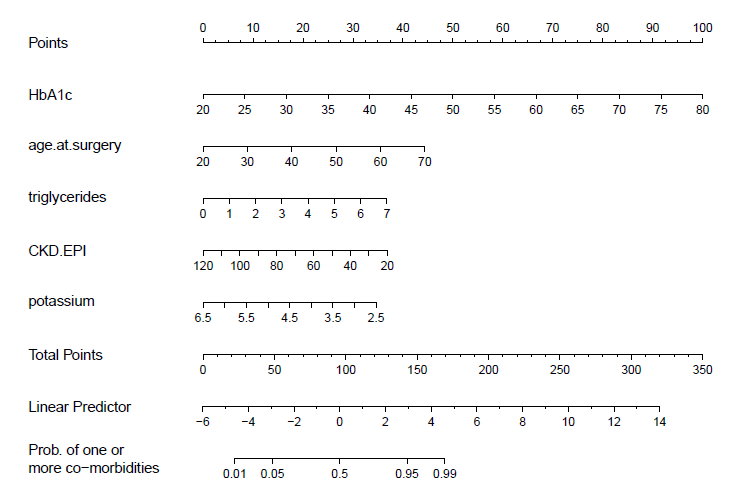
\includegraphics[scale=0.8]{BariatricNomogram.png}
%		\caption{The nomogram that explained the created comorbidity severity score of bariatric patients.\cite{Deneer2017Thesis}}
%		\label{fig:BariatricNomogram}
%	\end{figure}
	
	
	\subsection{Skin Diseases Data sets}
	\label{subsect:SkinDiseasesDataSet}
	
	% Introduction
	Skin diseases could form a major disability in someone's life. Whereas skin diseases were not as life threatening as diseases such as Cancer, Alzheimer and AIDS, the could lower quality of life significantly. When looking at health-related quality of life (HRQL), patients with psoriasis showed same problems as patients with other major chronic health conditions.\cite{rapp1999psoriasis} Patients with both psoriasis and eczema suffered from severe itching symptoms and possibly even severe pains. Further insights in these skin diseases could help alleviate their unwanted side-effects and help improve the patients' quality of life.\cite{jowett1985skin}
	
	% Data set introduction
	Information on both of these skin diseases could be found from nine data sets. The data sets consisted of information on skin of patients with the disease (lesional skin) and skin without the disease (non-lesional skin). In several experiments this skin was taken from the same patient. Also some skin was taken from patients not suffering from the diseases at all. Six data sets focused on Psoriasis and three focused on atopic dermatitis. These data sets consisted of a total number of 54675 features, each of them corresponding to a specific gene. Not many skin samples were taken, ranging from 28 to 180. Also, since every data set was created by different people, some minor differences were present in them as well (Table \ref{tab:SkinDiseasesDataSets}).
	
	\begin{table}[h!]
		\centering
		\caption{Details of the nine skin disease data sets. The number of samples and features has been given, as well as remarks of the skin types.}
		\label{tab:SkinDiseasesDataSets}
\begin{tabular}{cc|ccl}
	\textbf{Disease}                                                     & \textbf{Data set name} & \textbf{Sample size} & \textbf{Features} & \textbf{Remarks}                                                                                                                                                                                                                                        \\ \hline
	\textbf{Psoriasis}                                                   & \textbf{GSE13355}\cite{nair2009genome}      & 180                  & 54676             & \begin{tabular}[c]{@{}l@{}}Three skin types: \\ - NN (normal, 64 samples)\\ - PN  (non-lesional, 58 samples) \\ - PP (lesional, 58 samples)\end{tabular} \\ \cline{3-5} 
	\textbf{}                                                            & \textbf{GSE30999}\cite{suarez2012expanding}      & 170                  & 54676             & \begin{tabular}[c]{@{}l@{}}- No normal patients\\ - Non-lesional (85 samples)\\ - Lesional (85 samples)\end{tabular}                                                                                                                    \\ \cline{3-5} 
	\textbf{}                                                            & \textbf{GSE34248}\cite{bigler2013cross}      & 28                   & 54676             & \begin{tabular}[c]{@{}l@{}}- No normal patients\\ - Non-lesional (14 samples)\\ - Lesional (14 samples)\end{tabular}                                                                                                                              \\ \cline{3-5} 
	\textbf{}                                                            & \textbf{GSE41662}\cite{bigler2013cross}      & 48                   & 54676             & \begin{tabular}[c]{@{}l@{}}- No normal patients\\ - Non-lesional (24 samples)\\ - Lesional (24 samples)\end{tabular}                                                                                                                               \\ \cline{3-5} 
	\textbf{}                                                            & \textbf{GSE78097}\cite{kim2016spectrum}      & 33                   & 54676             & \begin{tabular}[c]{@{}l@{}}Different types of skin samples: \\ - Normal (6 samples)\\ - Mild Psoriasis (14 samples) \\ - Severe Psoriasis (13 samples)\end{tabular}                                                                                \\ \cline{3-5} 
	\textbf{}                                                            & \textbf{GSE14905}\cite{yao2008type}     & 82                   & 54676             & \begin{tabular}[c]{@{}l@{}}- Normal skin (21 samples), \\ - Non-lesional skin (28 samples)\\ - Lesional skin (33 samples)\end{tabular}                                                                                                                 \\ \hline
	\textbf{\begin{tabular}[c]{@{}c@{}}Atopic\\ Dermatitis\end{tabular}} & \textbf{GSE32924}\cite{suarez2011nonlesional}      & 33                   & 54676             & \begin{tabular}[c]{@{}l@{}}- Normal skin (8 samples) \\ - Non-lesional skin (12 samples)\\ - Lesional skin (13 samples)\end{tabular}                                                                                                         \\ \cline{3-5} 
	\textbf{}                                                            & \textbf{GSE27887}\cite{tintle2011reversal}      & 35                   & 54676             & \begin{tabular}[c]{@{}l@{}}Different type of skin samples, \\ pre and post treatment of skin: \\ - Pre non-lesional (8 samples)\\ - Post non-lesional (9 samples)\\ - Pre lesional (9 samples)\\ - Post lesional (9 samples)\end{tabular}       \\ \cline{3-5} 
	\textbf{}                                                            & \textbf{GSE36842}\cite{gittler2012progressive}      & 39                   & 54676             & \begin{tabular}[c]{@{}l@{}}Also difference between \\ acute and chronic dermatitis. \\ - Normal (15 samples)\\ - Non-lesional (8 samples) \\ - Acute lesional (8 samples) \\ - Chronic lesional (8 samples)\end{tabular}                    \\ \cline{1-5} 
\end{tabular}
\end{table}

	% Introduction challenges
	The nine data sets are rich in information. The dimensionality is very high and if combined also houses a decent number of samples. Several challenges arise in the data set, too, as biomedical data sets often have (subsection \ref{subsec:BiomedicalData}). Three of these challenges are discussed for this case.
	
	% Challenge 1: Data heterogeneity
	At first the challenge of handling nine different data sets was important. Even though the sets were created based on the NCBI database\cite{edgar2002gene}, the layouts were not identical. These difference originated from the intended research goals and the data availability. It is not possible to just concatenate samples without some form of preprocessing. Only the parts that are the same all over the data sets should be taken and all other parts omitted. A first look would be best on the nine data sets separately so initial ideas found with as less bias from combining them as possible.
	
	% Challenge 2: Data dimensionality
	A second challenge could be found in the high number of features. There were 74676 featured measured, averaged a 1000 times the number of samples. The genes that actually were significanlty involved in the skin diseases however should be about $1/1000^{th}$ of the total number of measured genes. Many features should be redundant and removed during preprocessing, a valuable and complex step in biomedical data mining.
	
	% Challenge 3: Data Quality
	 The third challenge was about data quality. The data was gathered from eight different groups with different standards. Some groups had taken the lesional and non-lesional skin from the same patient, whereas others did not. Also, there might also be different conditions per experiment, for example different measuring equipment. This could mean that the data would be more set specific and create bias in the data. This all diminished the quality, something that could hinder finding results in the process

	\subsection{Automated Machine Learning}
	\label{subsec:AutomatedMachineLearning}
	
	% History autoML
	Before automated machine learning (autoML) existed, a dataset was mined by hand. First a preprocessing algorithm was chosen and used to prepare the data. Next a (machine learning) algorithm was chosen to mine the desired results out of the data. At last the hyperparameters of the chosen algorithm were tuned to optimize the desired results. These three steps are vastly different and significant issues arise when combining these. Several ideas arose to combine the steps, called Combined Algorithm Selection and Hyperparameter optimization (CASH).\cite{thornton2013auto} After some time, when preprocessing was added in the mix as well, the name autoML was being used.\cite{Gijsbers2017Thesis} The first autoML approach tool was published as \texttt{Auto-WEKA} that focused on classification methods, spanning 2 ensemble methods, 10 meta-methods, 27 base classifiers and their hyperparameter settings.\cite{thornton2013auto} An upgrade was published that added regression and parallellism.\cite{kotthoff2016auto}   
	
	% Introduction to pipelines
	As explained shortly before, to go from data and results several steps must be taken: Preprocessing, algorithm selection and hyperparameter optimization. This sequencing is called a machine learning pipeline. Such a pipeline can consists of zero, one or multiple preprocessing steps for data preparation, can be one of many different machine learning algorithms which on their part have wide ranges for multiple hyperparameters. The explosion of possible pipelines makes it hard to choose the right one. Knowing successful combinations is useful, however every data set has different features that ask for different pipelines. \cite{Gijsbers2017Thesis}
	
	% Introduction autoML
	AutoML tires to find the best machine learning pipelines to compute which algorithms must be selected, combined with tuning the hyperparameters and preprocessing. This algorithm selection usually is done in a meta-learning approach, which focuses on finding how the machine learning algorithms perform for a task interval. Hyperparameter optimization has challenges on his own to find the right ones and there are many different approaches to tackle preprocessing. All of these are discussed in their own subsection to briefly explain them.	
	
	
	\subsubsection{Meta-Learning}
	\label{subsubsec:Meta-Learning}
	
	% Introduction meta-learning
	Machine learning algorithms show different behaviour for different tasks. Meta-learning tries to find out how their performance changes between those tasks (Figure \ref{fig:Meta-LearningLayout}). It tries to link the algorithm with data sets it would do good for and tries to find which hyperparameters give a good performance. In combination with the machine learning pipelines, meta-learning would try to find the best ones available. Since not only algorithms must be selected, but also hyperparameters must be optimized and preprocessing must be done, the time and space needed for meta-learning explodes. This can be lessened when removing bad pipelines and limiting the range of hyperparameters, machine learning- and preprocessing algorithms as much as possible. 

	\begin{figure}
		\label{fig:Meta-LearningLayout}
		\includegraphics[scale=1]{Meta-LearningLayout.png}
		\caption{A layout of how meta-learning works. 1. Data sets are collected. 2. Meta-data is computed for each dataset. 3. A meta-dataset is created and a meta-model is learned.\cite{Gijsbers2017Thesis}}
	\end{figure}
	
	% Meta-features
	Features of the meta-learning phenomenon are used to predict the performance. There are three types of these meta-features. The first type is simple, statistical and information-theoretic. They can be a basic feature of the data set, as well as a value after a statistical computation or a specific theoretical value. The second meta-feature type can be called landmarks. Landmarks give the performance of algorithms, how well they are doing with the given data set. The last meta-feature category is model-based. Specific characteristics of the used model can be used as meta-features as well.\cite{brazdil1994characterizing, vilalta2004using}

	% Meta-learners
	For using those meta-features in picking the best machine learning algorithm meta-learners can be used. Meta-learners are algorithms that choose between the possible choices. There are four ways of doing that. The first is plainly choosing the best algorithm in the set, this choice speeds up the process but is prone to being a bad choice. Second a subset of good algorithms can be chosen, which is slower, but has a higher chance to give a good outcome. Thirdly the algorithms can be ranked, which makes the chance of picking a good algorithm quicker starting at the top. Fourth is to use estimations of performance which gives information expectations over all algorithms.\cite{brazdil2009development}

	\subsubsection{Hyperparameter Optimization}
	\label{subsubsec:Hyperparameter optimization}

	% Introduction to hyperparameters
	As discussed before, machine learning algorithms have hyperparameters. These type of parameters are very sensitive and can change the algorithm performance greatly, hence the hyper- prefix. These hyperparameters can be nonlinear and nonconvex which results in it being hard to find the optimal value. They are many different variable types of hyperparameters, which makes standardizing optimization hard. They can also be dependent on each other and therefore have useless combinations. At last they can change the computation time drastically for a minor change in parameter.\cite{claesen2015hyperparameter}

	% Ways to find the right parameters
	There are several approaches to find the right values for the hyperparameters. Three approaches will be discussed. At first there is grid search, that checks all possible combinations for hyperparameters on a predefined interval. This approach does effectively check the complete area the optimal solution can be in, however it also takes much computational time due to the combinatorial explosion principle.\cite{hsu2003practical} A second approach is the random search, when values are chosen for each hyperparameter at random. It is proven that this search is better in an empirical and theoretical way, due changing some hyperparameters hardly making any difference.\cite{bergstra2012random} 
	
	% Bayesan optimization
	A more advanced way of optimizing hyperparameters is Bayesian Optimisation. This hyperparameter optimization approach tries to use earlier results to find the best possible location for the hyperparameters to be optimized. At the start, with random sampling several sample points are measured. An acquisition function, with the input from earlier samples, which combination of hyperparameters should be tested next. It balances between trying to explore areas with good performance and trying to explore bigger areas for possible other good areas.\cite{snoek2012practical} The three optimization techniques are shown together to explain the difference (Figure \ref{fig:HyperparameterOptimization}).
	
	\begin{figure}
		\label{fig:HyperparameterOptimization}
		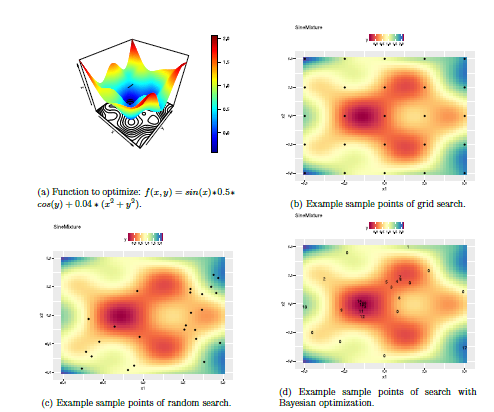
\includegraphics[scale=0.8]{HyperparameterOptimization.png}
		\caption{Examples of the three explained hyperparameter optimization techniques. The numbers in the bayesan optimization show the iteration of sampling.\cite{Gijsbers2017Thesis}}
	\end{figure}
	
	\subsubsection{Preprocessing}
	\label{subsubsec:Preprocessing}
	
	% Introduction preprocessing
 	Preprocessing is one of the three aspects of autoML. Whereas the goal is important when choosing a type of machine learning algorithm, preprocessing algorithms always need to be fine-tuned for the available data set, as every set is different. Data sets, and specially biomedical ones for this project, have specific challenges that can be solved using preprocessing (subsection \ref{subsec:BiomedicalData}). These challenges can be classified in two regions. The first one is about problems with the data, The second one is data preparation.\cite{famili1997data}
 	
 	% Too much data
 	From a preprocessing point of view, there can be three different types of problems with data (Figure \ref{fig:DataPreprocessing}). The first problem is that there is too much data. The data can be noisy, irrelevant, too big, different types of data can be present and feature extraction still has to be done. The data for this project is an example for noisy data (subsection \ref{subsec:BiomedicalData}), as 5\% of the data is estimated to be wrong.
 	
 	% Too little data
 	A second type is the opposite of having too much data. There can also be too little data. Values of an attribute or complete attributes can be absent from the data. The number of data points can also be very low. For the example data set, there were many cases where attributes were missing.
 	
 	% Fractured data
	A third problem with the data can be that it is fractured. Multiple separate data sets can be incompatible, come from multiple sources or are on different processing levels. When taking the bariatric data as an example, it stems from two different data sets. A challenge is to combine these two as one data set, as one, while they are not specifically made for that.
 	
	% Data preprocessing techniques/Data transofmration
	To tackle those three data problems, again three types of techniques can be used. At first data can be transformed to become more usable. The most important transformation is noise removal. It can be removed with smoothing function\cite{somorjai2004data, karagiannis2011noise}, or a more advanced machine learning technique to also detect it.\cite{gamberger2000noise}
 	
 	% Information gathering
 	A second preprocessing technique is gathering data if needed. Data selection is important, as it could be that not all data is as relevant as all the other data. Important techniques to be mentioned are principal component analysis, that checks the relevance for every feature in the data set.\cite{duszak1994using} 
 	
 	% Generation of new information
 	At last new information can be generated, if needed. This can be done by simulation or by adding new features. Data points can be fused to become a new point. This way more data is available for data analysis. Also when values are missing, several techniques can be used for value imputation. Extrapolation can be done, using regression to estimate its value. Other methods are based on nearest neighborhood frameworks.\cite{zhu2011missing} 
 	
 	\begin{figure}[h!]
 		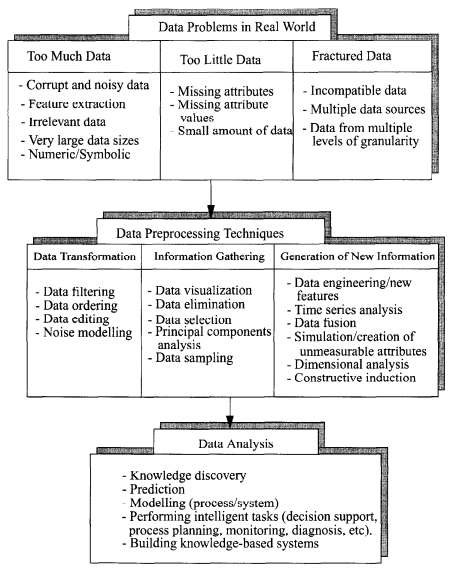
\includegraphics[scale=1]{DataPreprocessing.png}
 		\caption{A schema that shows the process of preprocessing.\cite{famili1997data}}
 		\label{fig:DataPreprocessing}
 	\end{figure}
 	
 	% Rawness challenges
 	Aside from data problems, another reason for preprocessing can be present.\cite{famili1997data} Data can also be very raw. STo reach a certain goal, a data set has the necessary iformation, but only indirectly. An example would be hypertension. To know if someone has hypertension, its blood pressure must be measured and checked if that value is high enough. this preprocessing is highly data set specific, as computers do not know the specifications of blood pressure for someone having hypertension. 
 	
	\subsection{Tree-based Pipeline Optimization Tool}
	\label{subsec:TPOT}
	
	% Introduction TPOT
	A tool that implements autoML is tree-based pipeline optimization tool (TPOT). It uses the machine learning pipelines and evolutionary optimization to find the best solution for every data set. This evolutionary optimization is done by genetic programming. Genetic programming evolves possible solutions to find a better solution. This evolution is done by first evaluating them and selecting the best ones to continue to the next generation. Then both crossovers between and mutations on possible solutions are performed. After that again evaluation and selection, followed by crossovers and mutations, take place a number of times until a certain quality is found, time has run out or another ending condition has been met.
	
	% TPOT layout
	TPOT makes use of this genetic programming with using the machine learning pipelines in a tree (Figure \ref{fig:MachineLearningPipeline}). TPOT consists of preprocessing and machine learning algorithms, that form the backbone of the pipelines. Their hyperparameters and the data set are the variables. TPOT makes mostly use of the machine learning and preprocessing algorithms of skikit-learn from Python in which it is also written.
	
	\begin{figure}[h!]
		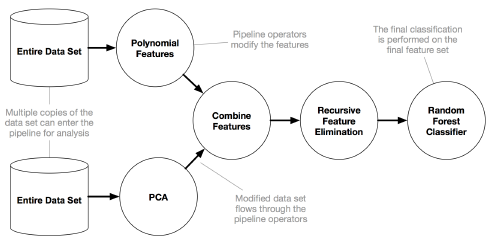
\includegraphics[scale=1]{MachineLearningPipeline.png}
		\caption{An example of a machine learning pipeline in TPOT. It only shows the primitive algorithms and not hyperparameter terminals. At the root is the machine learning algorithm.\cite{Gijsbers2017Thesis}}
		\label{fig:MachineLearningPipeline}
	\end{figure}

	% TPOT mutation operators
	TPOT has three different types of mutations within one pipeline.The first one is insertion, inserting a primitive somewhere in the tree. An example would be the insertion of an additional preprocessing algorithm. The second one is replacement, which replaces a random terminal. It can for example change a binary hyper parameter from true to false. The third one is shrinking. A primitive is replaced by a terminal. For example a preprocessing step can be replaced by just raw data. This different mutations can all be seen visually (Figure \ref{fig:TPOTMutations})
	
	\begin{figure}[h!]
		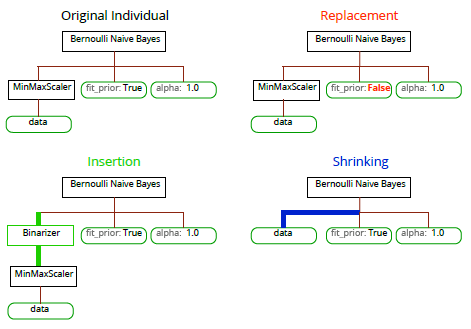
\includegraphics[scale=1]{TPOTMutations.png}
		\caption{Examples of the three mutations in the TPOT algorithm: insertion, replacement and shrinking.\cite{Gijsbers2017Thesis}}
		\label{fig:TPOTMutations}
	\end{figure}
	
	% Crossover
	TPOT also focuses on mutations between two pipelines through the means of crossovers. Between two pipelines, sub-trees and primitives can be changed, given that the both pipelines remain valid (Figure \ref{fig:TPOTCrossover}). Every time a crossover is performed, two separate pipelines are used and changed, creating two new ones.
	
	\begin{figure}[h!]
		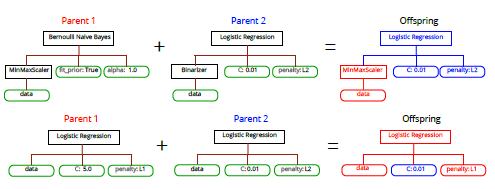
\includegraphics[scale=1]{TPOTCrossover.png}
		\caption{An example of a TPOT crossover\cite{Gijsbers2017Thesis}}
		\label{fig:TPOTCrossover}
	\end{figure}
	
	% Biomedical preprocessing
	Comparing the possibilities from TPOT and the challenges in biomedical data, it seems that TPOT has some implementations to tackle them. It has several different scalers (StandardScaler, RobustScaler, MinMaxScaler) to tackle feature heterogeneity between different data sets and errors. It also has some feature selection operators to tackle errors (VarianceThreshold, SelectKBest, SelectPercentile). For missing values, the algorithm imputes the median as estimation for the missing value.
	
	\section{Research Question}
	\label{sec:ResearchQuestion}
	
	%Introduction research question
	TPOT has shown to give promising results for several different data sets.\cite{Gijsbers2017Thesis} For this project the focus will be on biomedical data sets (subsection \ref{subsec:BiomedicalData}) and how it handles specific problems in these data sets. An example data set (subsection \ref{subsect:SkinDiseasesDataSet}) is taken for analysis and to create suggestions for future extensions of TPOT. The research question for TPOT will be the following.\\
	
	How does TPOT perform on specific biomedical data set problems and how can it be improved on them?\\
	
	\subsection{Hypothesis}
	\label{subsec:Hypothesis}
	
	% Hypothesis
	Knowing that some algorithms exist to tackle the problems with biomedical data sets, the first step should be to find out whether TPOT can process the data set without any problems. It is expected to succeed in that, as TPOT showed good results for nono-biomedical data sets. The skin disease data set (subsection \ref{subsect:SkinDiseasesDataSet}) had three biomedical data challenges: data heterogeneity, high dimensionality and data quality. These challenges are discussed separately

	% Challenge 1
	With regards to data heterogeneity, TPOT has no ways to use multiple data sets as an input and aligning them. This needs to be done manually by preprocessing. 
	
	% Challenge 2
	TPOT has ways to tackle high dimensionality with preprocessing. Principal Components Analysis (PCA), Feature Agglomeration, Independent Components Analysis (ICA), Recursive Feature Eliminations (RFE) are four examples of dimensionality reduction. These dimensionality reductions are often used in biomedical data analysis and could prove useful. A benefit of these methods to reduce high dimensionality is the simplicity to extract important genes from the pool after being preprocessed. Other ways TPOT tackles the high dimensionality is with several machine learning techniques as decision trees and random forests. These techniques filter out the best genes for classifications.
	
	% Challenge 3
	The third challenge was about data quality. Since the data stems from different experiments, bias should be present. This bias can be tackled by some forms of preprocessing that are available in TPOT. Examples are using normalizers, several types of scalers, thresholds and binarizers. These preprocessors are done only after merging the data sets though, which could hinder the effectivity. This challenge would not be tested on specifically, however could hinder the final scoring of pipelines.
	
	% Summary
	All things considered TPOT should be able to handle several biomedical data set challenges sufficiently, whereas others are probably not present at all. Future development can be suggested to improve TPOT and have it sufficiently tackle those biomedical data problems, as well.
	
	\section{Methods}
	\label{sec:Methods}
	
	% Introduction Methods
	The approach to answer the research question was split in three different parts. At first preprocessing was done to align the nine data sets as much as possible. Secondly the data sets were used as input in the TPOT classifier to find the best possible pipeline and some analysis was done to evaluate that. Third and last the data set was combined as much as possible and run through the model again. 
	
	% Software
	All programming in this project has been done using Python, with the help of anaconda. TPOT was written in python and therefore using Python would seriously reduce compatibility issues. Anaconda was used for for the same reasons, as with anaconda it is fairly simple to import packages used by TPOT and packages that are imported for preprocessing and analysis. Jetbrains Pycharm was used as an environment mainly because of coding assistance and previous experience with it.
	
	
	% Hardware
	For running the experiments only a cpu was available. This meant that memory issues could be present. After some testing on basic data sets (e.g. MNIST), memory gave no issues and was not expected to give issues after using data sets of a similar size.
	
	\subsection{Preprocessing}
	\label{subsec:Preprocessing}
	
	% Introduction preprocessing
	Preprocessing was a big part of the project. Even though all data was generated with the NCBI database\cite{edgar2002gene} in mind, the raw data had to be pruned and all of them in a different way. This pruning consisted of removing irrelevant data, extracting essential data and prepraring it for tpot to use. 
	
	% Downloading data
	To download the data, the NCBI database was used (Table \ref{tab:SkinDiseasesDataSets}).  An advantage of the NCBI database is that the data is made available in different file types. The base type is a  \textit{.cel} type and all other types were based on that one. Other types were \textit{SOFT}, \textit{MINiML} and also just a regular matrix (\textit{.txt}) file. Since only a matrix with the data and type of skin for each sample was needed, the most basic (\textit{.txt}) file was used. Nine different (\textit{.txt}) files were downloaded from the database and stored for preprocessing
	
	% Removing irrelevant data
	The data was one big matrix with for every row an undetermined number of columns. The rows could be split into four different parts: title, set attributes, sample attributes and experiment values. Each part had their own starting row followed by one specific attribute every row. Therefore at first the data was split into these four sections, so further pruning could be done on every section separately. The title and set attributes only consisted of information how to manually locate relevant data locations. Therefore after reading them, these two parts were discarded for future preprocessing.
	
	% Extracting relevant data
	The sample details contained several attributes for every sample. This part consisted of much irrelevant data, as well, with the exception of skin type. This skin type therefore needed to be extracted first before discarding this part. This skin type had to be manually extracted out of every sample title, as no attribute for skin type was present. The experiment values were more straightforward. The first row consisted of the sample IDs, that could be linked to the sample IDs of the sample details. Every following row consisted of a specific gen as well as the values of every sample.
	
	% Preparing data
	Preparation of the data was minor due to efficient data extraction. The experiment values were extracted as a matrix and therefore immediately available for the TPOT classifier. For the skin types, three categories were made and a list was made with those categories, corresponding to the samples and their experiment values. The data sets and available skin types (table \ref{tab:SkinDiseasesDataSets}) were mapped as good as possible on the list: 
	
	\begin{enumerate}
		\item[(0)] Normal skin. The normal skin values were extracted from patients not suffering from a skin disease. In case of no mention whether skin was normal or non-lesional, it was expected to be normal
		\item[(1)] Non-lesional skin. Skin of a skin disease patient not affected by it.
		\item[(2)] Lesional skin. Skin of a skin disease patient that is affected by it.
		\item[(3)] Dummy variable. Variable specific for that data set that is not compatible with the others
	\end{enumerate}

	% Mapping mismatches
	Not all data sets could efficiently be mapped. The 'GSE78097' set had two types of lesional (mild and severe) and no normal skin. The 'GSE27887' had pre- and post treatment non-lesional and lesional skin. For both of these sets, a manual ordering was made, so these data sets should be treated differently when combined
	
	
	\subsection{TPOT}
	\label{subsec:MethodsTPOT}
	
	% Creating training and test set
	After the data sets had been preprocessed, they were available for TPOT calculations. The experimental values and skin types should be used as input for the TPOT classifier whereas the values are the input features and the skin types the output. Before actually using the data, first it should be split into a training and test set. Even though TPOT itself also uses a training and test set to prevent overfitting of data, a small test set still was used to calculate the score on data TPOT had not seen itself, yet. Since the number of samples was very low to begin with, only 0\% of the data was regarded as training data and only 10\% as test data.
	
	% TPOT setup
	 Since classification was needed, the TPOT classifier was used which made use of several algorithms. These algorithms were mostly borrowed from sklearn and some were created by TPOT itself (Table \ref{tab:TPOTAlgorithms}). Before using TPOT, several parameters had to be selected. The selected parameters all revolve around the genetic algorithm used for selecting the best machine learning pipeline (subsection \ref{subsec:AutomatedMachineLearning}):
	 
	 \begin{enumerate}
	 	\item[-] \textit{generations}, the number of generations the genetic algorithm should run before terminating. If the number of generations had been reach the TPOT classifier ended. the number of generations was set on 100.
	 	\item[-] \textit{population\_size}, the number of pipelines that needed to be stored for further generations. After every generation the worst pipelines were discarded. The number of modifications was also linked to the number of modifications to the pipelines, so every generations 10 modifications were made. The population size was set on 10.
	 	\item[-] \textit{max\_time\_mins}, the time limit the TPOT classifier is allowed to find the best pipeline. If it still runs when the time limit has been reached it will end pre-emptively. Due to severe time constraints, the time limit was set on 120 minutes. 
	 \end{enumerate}
	
\begin{table}[]
	\centering
	\caption{All TPOT Algorithms used for the TPOT classifier function. Not only the algorithms differ, but also the hyperparameters within these algorithms.}
	\label{tab:TPOTAlgorithms}
	\begin{tabular}{ll|l}
		\textbf{Algorithm type} & \textbf{Specification}  & \textbf{Algorithms}                                                                                                        \\ \hline
		\textbf{Classifier}     & Naïve Bayes             & GaussianNB, BernoulliNB, MultinomialNB                                                                                     \\
		\textbf{}               & Decision Tree           & \begin{tabular}[c]{@{}l@{}}DecisionTree, ExtraTrees, RandomForest, \\ GradientBoosting\end{tabular}                        \\
		\textbf{}               & Nearest Neighbor        & KNeighbors                                                                                                                 \\
		\textbf{}               & Support Vector Machines & LinearSVC                                                                                                                  \\
		\textbf{}               & Logistic Regression     & Logistic Regression                                                                                                        \\ \hline
		\textbf{Preprocessors}  & Scaler                  & \begin{tabular}[c]{@{}l@{}}Binarizer, MaxAbsScaler, MinMaxScaler, \\ Normalizer, RobustScaler, StandardScaler\end{tabular} \\
		\textbf{}               & Feature reduction       & \begin{tabular}[c]{@{}l@{}}PCA, FastICA, RBFSampler, Nystroem,\\ FeatureAgglomeration\end{tabular}                         \\
		\textbf{}               & Feature Modifier        & Polynomial, OneHotEncoder,ZeroCount                                                                                        \\
		\textbf{}               & Feature Selectors       & \begin{tabular}[c]{@{}l@{}}SelectFwe, SelectPercentile, VarianceThreshold, \\ RFE, SelectFromModel\end{tabular}           
	\end{tabular}
\end{table}
		
	% Pipeline storage
	After the best pipelines had been chosen, they were stored in a separate file. These files consisted of both the chosen algorithms and their hyperparameters as well as the score after fitting the test size on it. Since TPOT only chose the best possible pipeline, if it would be used it should be fitted another time for the data set for further calculations.
		
	% Introduction analysis
	To analyse the created pipelines, every data set was fitted on every pipeline. Again a training and test set was created to find out how well the pipelines would behave for very data set. The acquired score could be used to show how well that pipeline would behave for every data set. Every data set was fitted 10 times and the acquired scores were averaged to better represent the actually quality of the pipeline.
	
	\subsection{Data Set Combination}
	\label{subsec:MethodsDataSetCombination}
	
	% Introduction data set combination
	At last all possible data sets were combined to create one big data set with more samples. Since not all of them were applicable to add, only the data sets with the names 'GSE13355', 'GSE30999', 'GSE34248', 'GSE41662' and 'GSE14905' were chosen. Psoriasis data sets were chosen instead of atopic dermatitis simply because more of those were available. After combining these data sets the final number of samples was 508 with the following distribution:
	
	\begin{enumerate}
		\item[-] \textit{Normal skin:} 85 samples
		\item[-] \textit{Non-lesional skin:} 209 samples
		\item[-] \textit{Lesional skin:} 214 samples
	\end{enumerate}

	% Running in TPOT
	To run this with TPOT classifiers new input parameters should be chosen. Since this data set was about three times larger than the largest data set run so far and the differences between data sets had to be overcome as well, a larger running time had to be given for this case. The following parameters were given:
	
	 \begin{enumerate}
		\item[-] \textit{generations:} 100
		\item[-] \textit{population\_size:} 40
		\item[-] \textit{max\_time\_mins:} 480 
	\end{enumerate}

	% Analysis
	After the TPOT classification had been run, it was analysed for the data set. This was done by fitting it ten times and averaging the acquired scores. The eight original pipelines were all being fitted for the data set the same way, to find out if they still produced good results with more data points from different data sets.

	
	\section{Results}
	\label{sec:Results}
	
	%Introduction results
	The results were split into two parts. Since preprocessing did not have any results to be presented (the preprocessed dataset itself was the result), only TPOT and combination of the data sets were presented.
	
	\subsection{TPOT}
	\label{subsec:ResultsTPOT}

	% Problems TPOT
	Before acquiring the results there were several problems with using the data set in TPOT. At first several TPOT algorithms had trouble with using several algorithms on the high dimensional data set. Some required almost all memory making the TPOT classifier much slower than needed. The preprocessing algorithm \textit{FeatureAgglomeration} even froze the computer, requiring it to restart. Therefore this algorithm was manually removed from all possibilities in the TPOT classifier. The data set 'GSE36842' also had problems finding an optimal pipeline because of unknown reasons and therefore was also removed from the pipeline selection.
	
	% Results TPOT
	The results for the eight remaining data sets were different from each other (Table \ref{tab:ResultingPipelines}). In all cases the running time was the biggest constraint, so new runs should be done in longer time. The most picked classifier seemed to be \textit{RandomForestClassifier}, being picked three times to find possible better results. The hyperparameters did not seem very similar for these three though. \textit{LinearSVC} was also picked twice, with different hyperparameters. Interestingly enough a preprocessing algorithm was used only once, which was the \textit{Binarizer} algorithm. This preprocessing alogrithm was not a feature reduction algorithm, while those algorithms were more expected to be present in the final pipelines. Looking at final scores of these pipelines, most of them were close to a perfect score, two of them even being a perfect classification score. Data sets 'GSE13355' and 'GSE32924' settled for a far lower score around $0.83$ and for data set 'GSE27887'a score of only $0.51$ was the best the TPOT classifier could find.

\begin{table}[h!]
	\centering
	\caption{All discovered pipelines with the TPOT classifiers for the mentioned data sets as well as the scores for those pipelines. The sample size is given for comparison, too.}
	\label{tab:ResultingPipelines}
	\begin{tabular}{c|c|c|r}
		\textbf{Data set} & \textbf{Sample size} & \textbf{Score}     & \multicolumn{1}{c}{\textbf{Pipeline}}                                                                                                                                                                                                \\ \hline
		\textbf{GSE13355} & 180                  & 0.8333793341383474 & \begin{tabular}[c]{@{}r@{}}Binarizer(threshold=0.7)\\ RandomForestClassifier(bootstrap=False, \\ criterion="entropy", \\ max\_features=0.35, \\ min\_samples\_leaf=3, \\ min\_samples\_split=18, \\ n\_estimators=100))\end{tabular} \\ \hline
		\textbf{GSE30999} & 170                  & 0.9804301075268818 & \begin{tabular}[c]{@{}r@{}}KNeighborsClassifier(n\_neighbors=9, \\ p=2, \\ weights="distance")\end{tabular}                                                                                                                          \\ \hline
		\textbf{GSE34248} & 28                   & 0.9666666666666668 & \begin{tabular}[c]{@{}r@{}}RandomForestClassifier(bootstrap=True, \\ criterion="entropy", \\ max\_features=0.9, \\ min\_samples\_leaf=3, \\ min\_samples\_split=6,\\  n\_estimators=100)\end{tabular}                                \\ \hline
		\textbf{GSE41662} & 48                   & 1.0                & \begin{tabular}[c]{@{}r@{}}LinearSVC(C=0.001, \\ dual=True, \\ loss="hinge", \\ penalty="l2", \\ tol=0.01)\end{tabular}                                                                                                              \\ \hline
		\textbf{GSE78097} & 33                   & 1.0                & \begin{tabular}[c]{@{}r@{}}RandomForestClassifier(bootstrap=False, \\ criterion="gini", \\ max\_features=1.0, \\ min\_samples\_leaf=4, \\ min\_samples\_split=10,\\  n\_estimators=100)\end{tabular}                                 \\ \hline
		\textbf{GSE14905} & 82                   & 0.9733333333333334 & \begin{tabular}[c]{@{}r@{}}LinearSVC(C=5.0, \\ dual=True, \\ loss="squared\_hinge", \\ penalty="l2", \\ tol=0.001)\end{tabular}                                                                                                      \\ \hline
		\textbf{GSE32924} & 33                   & 0.8283333333333334 & \begin{tabular}[c]{@{}r@{}}GradientBoostingClassifier(learning\_rate=1.0, \\ max\_depth=8, \\ max\_features=0.75, \\ min\_samples\_leaf=4, \\ min\_samples\_split=3, \\ n\_estimators=100, \\ subsample=0.7)\end{tabular}            \\ \hline
		\textbf{GSE27887} & 35                   & 0.5142857142857142 & \begin{tabular}[c]{@{}r@{}}DecisionTreeClassifier(criterion="gini", \\ max\_depth=4, \\ min\_samples\_leaf=1, \\ min\_samples\_split=10)\end{tabular}                                                                               
	\end{tabular}
\end{table}

	% Results analysis
	Since the data sets were similar. The data sets were tested on each other multiple times to find out which pipeline worked best on which data set (Figure \ref{fig:DataPipelineScores}). Those scores showed that no pipeline is best for any data set. Furthermore, they showed that even after trying different pipelines, they show very similar behaviour. For almost every data set no clear best or for example top three could be chosen. 
	
	\begin{figure}[h!]
		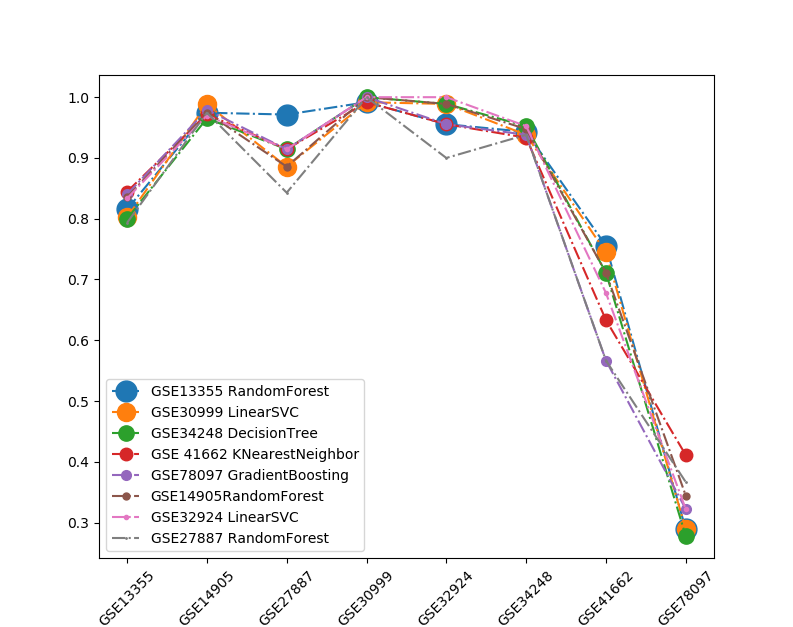
\includegraphics[scale=0.6]{DataPipelineScores.png}
		\caption{The scores of the pipelines after fitting them on every data set.}
		\label{fig:DataPipelineScores}
	\end{figure}

	\subsection{Data Set Combination}
	\label{subsec:ResultsDataSetCombination}
	
	% Introduction TPOT combinations
	Also when combining the data set combinations, TPOT stopped trying to find the best pipeline after the time limit has been reached. The time limit should be a factor $10^2$ higher it seems to fit the number generations. The final pipeline was the following:
	
	\begin{enumerate}
		\item[] \textit{Best pipeline:}  LogisticRegression(C=0.0001, dual=True, penalty='l2'),
		GradientBoostingClassifier(learning\_rate=0.1, max\_depth=5, max\_features=0.05,
		min\_samples\_leaf=12,
		min\_samples\_split=19, n\_estimators=100, subsample=0.5)
		
	\end{enumerate}

	% Discussing this pipeline
	The best pipeline being a combination of logistic regression and gradient boosting classifier seems like a plausible best pipeline. Both are often used for high dimensional data. Also, when looking at the hyperparameters of the gradient boosting classifier, the decision trees made for it can become quite big (a minimum of 5 depth and 12 leaf nodes). The logistic regression could make choices for the decision tree easier.
	
	% Analysis
	The score for the newly created pipeline is 0.913725490196. This score is not as high as the score for some data sets separately, which can be explained by the bias entered when combining them. The score has a high success rate, though, so it definitely is not bad. The pipelines created for the original data sets were also checked for the combined set to find a difference (Table \ref{tab:ScoresCombinedPipelines}). These show that the final created data set did show better results.
	
	\begin{table}[h!]
		\centering
		\caption{The scores when using the pipelines from the separate data sets with the combined set. The score for their own data set set are added as well as the algorithms used.}
		\label{tab:ScoresCombinedPipelines}
		\begin{tabular}{l|lll}
			\textbf{Data set} & \textbf{Algorithms}                                              & \textbf{Own score} & \textbf{Combined Data set score} \\ \hline
			\textbf{GSE13355} & \begin{tabular}[c]{@{}l@{}}Binarizer\\ RandomForest\end{tabular} & 0.8333793341383474 & 0.674509803922                   \\
			\textbf{GSE30999} & KNearestNeighbor                                                 & 0.9804301075268818 & 0.860784313725                   \\
			\textbf{GSE34248} & RandomForest                                                     & 0.9666666666666668 & NOG NIET BEKEND                  \\
			\textbf{GSE41662} & LinearSVC                                                        & 1.0                & NOG NIET BEKEND                  \\
			\textbf{GSE78097} & RandomForest                                                     & 1.0                & NOG NIET BEKEND                  \\
			\textbf{GSE14905} & LinearSVC                                                        & 0.9733333333333334 & NOG NIET BEKEND                  \\
			\textbf{GSE32924} & GradientBoosting                                                 & 0.8283333333333334 & NOG NIET BEKEND                  \\
			\textbf{GSE27887} & DecisionTree                                                     & 0.5142857142857142 & NOG NIET BEKEND                 
		\end{tabular}
	\end{table}
	
	\section{Conclusion}
	\label{sec:Conclusion}
	
	% Conclusion based on research question
	To give an answer to the research question (section \ref{sec:ResearchQuestion}) how TPOT would perform with typical biomedical data set problems, a two sided answer should be given. It is able to cope with some data set problems, however also shows issues with them.
	
	% Memory issues
	A first issue came up when running the high dimensional data. TPOT had memory issues when using several algorithms, even concluding in one algorithm being excluded from the possible outcomes. With time being a constraint for finding the best possible pipeline, it is not desired that several options take much longer to compute. 
	
	% When already knowing several parts of the data, a more supervised look for the best pipeline could result in a more effective search. 
	
	% Low sample number
	Where on the one hand, the high dimensionality was an issue, the low number of samples seemed an issue, as well. Test sets could accidentally satisfy the fitted pipeline much easier when only a small subset was used. No really possibilities are available to tackle that. An example would be to create more samples using the known ones.
	
	% Data combination problem
	
	% Good actions TPOT 
	TPOT did, however find good pipelines. Five of the 8 data sets in the end had a pipeline with a scoring of (close to) 1. This means that it did succeed finding good pipelines for more than half of the data sets. This shows that there definitely is potential for TPOT to be used for biomedical data sets.
	
	% Concluding conclusion
	All things considered TPOT did perform reasonably well for these biomedical data sets. It showed results that are definitely usable for further research. When some more changes would be added to address memory issues, adding the options of choosing possible algorithms and adding the possibility of creating more samples, TPOT become a very good tool for biomedical engineers to use.
	
	\section{Discussion}
	\label{sec:Discussion}
	
	% Introduction discussion
	The biomedical world strongly benefits from using the advanced techniques created by the data mining world. These techniques usually enter the biomedical data analysis projects later, due to a gap between them. This can be achieved by creating better communication between the worlds, so the data miners understand and implement important aspects of the biomedical research and the biomedical engineers do the same with data mining techniques. Projects like this one help filling that gap. Continuing this more breakthroughs can be achieved for better understanding and treatments in the hospital.
	
	% Time constrains weighed heavily
	During this project time was a severe constraint. At first different data was supposed to be made available. This data was bariatric data from the Catharina Hospital in Eindhoven, which focussed on different biomedical data challenges.\cite{Deneer2017Thesis} When it became clear that it was not possible to have this data in time, new data had to be searched. This meant that the implementation phase of the project did start in January instead of November. On top of that, the preprocessing took up quite some time as did solving the memory issues and finding out which algorithm froze the cpu. Because of that the experiments were run much shorter than initially planned to run. This worsened the results as TPOT is not expected to successfully find an optimization. A future work on this project extending it for a period of time would be of great benefit.
	
	% Other biomedical data set issues
	Only a selection of biomedical data set issues were present for this skin disease data set. Issues such as data complexity, volume or different aspects of quality could be addressed with a different data set. A clinical data set with blood markers and manual subscriptions would be an example of a data set with quality challenges, whereas a data set with MRI images would be interesting for testing complexity. Future projects could be based around those.
	
	% No possibility to look at the features
	A last not discussed characteristic is showing the links between input with output. Creating a model that correctly links input and output is nice, however in the biomedical world there is more to it than only creating this model. For the skin disease data set it would be very helpful if the conclusion would have given several genes that were important for diagnosing psoriasis or atopic dermatitis. Those genes can be further tested in what way they stimulate the expression of those diseases to gain more insights to possibly find a remedies for that. Whereas some classification techniques clearly show which features were used (decision trees, random forests), others create a swamp in which it is much harder to find them (support vector machines). A possible extension for TPOT to address this characteristic would be very beneficial.
	
	\bibliography{../References/Citings} 
	\bibliographystyle{ieeetr}
	
\end{document}
\